\section{Results}
\subsection{Simplices}
The first set of topological statistics we look at are the simplices. These statistics describe the local connectivity of a random graph. The higher the dimension of a simplex and the more simplices observed in each dimension, the more complex the structure becomes. The higher the dimension of the simplex, the more ordered this structure becomes.

Beginning with the Bio-M MC, we observe large numbers of simplices across the dimensions that went as high as dimension 6. In dimensions 2 and 3, we see simplices of almost as many as 80 and 70 million respectively.

The first model of comparison is the \ER model. This model is able to match the simplicial counts of the Bio-M MC in the $0^{th}$ and $1^{st}$ dimensions, however, with a lack of order applied to the model, the complexity and ordered structure diminishes, the higher the simplicial dimension we attain.

The second model, the General Biological model, as produced here \cite{Reimann_2017}, again matches the Bio-M MC in the $0^{th}$ and $1^{st}$ dimension. The number of $2^{nd}$ dimensional simplices observed here is somewhat larger than what has been produced by the \ER model. There are approximately 35 million 2-dimensional simplices and just below 10 million 3-dimensional simplices. These two dimensions in particular are a focus point for which to be able to compare the four models proposed here.

The Configuration model, like all subsequent models, produced precisely the same number of $0^{th}$ and $1^{st}$ dimensional simplices as that of the \ER model and the General Biological model, since these describe a single vertex and a directed edge joining two vertices as part of an ordered set respectively. The first difference occurs with the 2-dimensional simplices. Of the four proposed models, the Configuration model produced, consistently, the fewest 2-dimensional simplices. We observed approximately 33.5 million each time, 3 million fewer than the General Biological model. There is almost the same difference in the number of simplices between the Configuration model and the General Biological model for simplices in the $3^{rd}$ dimension compared to the $2^{nd}$ dimension.

Applying the geometric constraint in the Geometric Configuration model saw an improvement in matching the complexity of the Bio-M MC for 2-dimensional and higher simplices when compared to the Configuration model and the General Biological model. This refinement in the model, allowed for the biggest jump in accuracy between models, showing as many as 5 million more 2-dimensional simplices than the Configuration model, and almost 3 million more in the $3^{rd}$ dimension.

The next model, the Block Configuration model saw the application of a biological constraint. This constraint is the layer to layer interactions of the neurons. By applying this layer to layer constraint, we were able to further improve the model's likeness to the Bio-M MC. This model observed as many as 41 million 2-dimensional simplices and 8.5 million 3-dimensional simplices. This is an improvement in both dimensions from the Geometric Configuration model.

The Block Geometric Configuration model produced a similar number of 2- and 3-dimensional simplices as the Block Configuration model. So, there was no significant improvement to the numbers in these dimensions. However, this model did produce some more complex simplicial structures. We observed simplices in dimensions as high as the $6^{th}$, matching that of the Bio-M MC, just not as numerous.

\begin{figure}[H]
\begin{center}
\captionsetup{justification=centering}
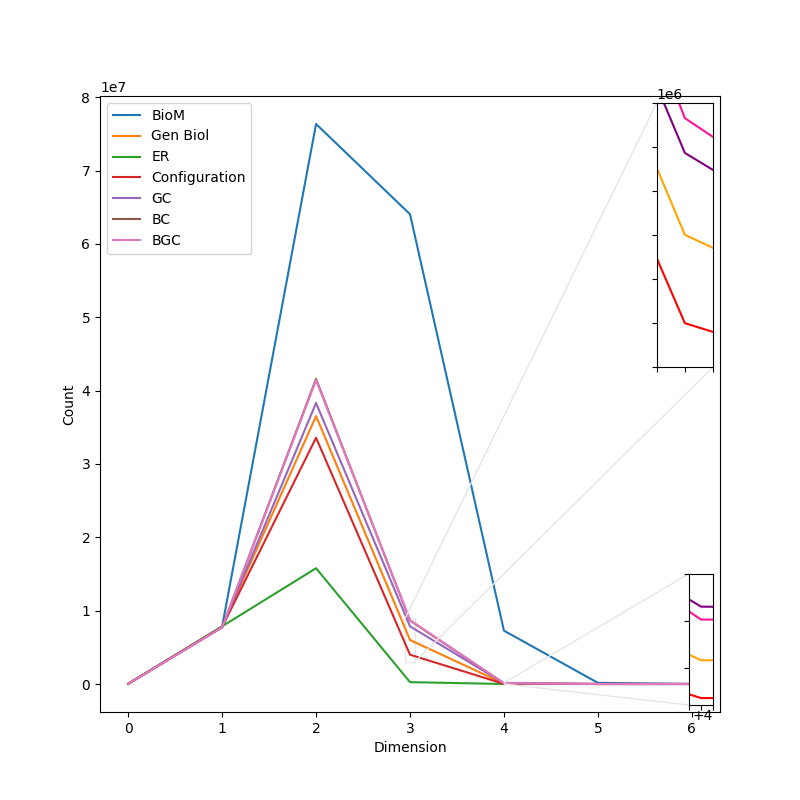
\includegraphics[height=8cm,width=12cm]{graph/simplices_zoomed.png}
\caption{Simplicial Comparisons}
\end{center}
\end{figure}



\subsection{Betti Numbers and Euler Characteristic}
We want to compare the global connectivity of each model. We do this with Betti Numbers. In particular, we want to compare this connectivity in the highest dimension for which each model observes a non-zero Betti Number. This occurs in dimension 3. We have below, a set of results for 100 realisations of each model to give ourselves a statistical range to work with.

In figures 40-42, we have individual box-plots for each model, followed by a box-plot with all the models side by side. The reason behind this can be observed with the scales used in each individual box-plot. We begin with the \ER model observing anywhere between 0 and 10 $3^{rd}$ dimensional Betti Numbers, all the way up to the Geometric model observing approximately $30,000$. Given that Betti Numbers is a count for the organisation of the structure of the graph, we can see that with a geometric constraint applied to the network, this enables the MC to maintain a lot more ordered structure than without this constraint. This appears more apparent between the Configuration model and the Geometric Configuration model than the respective Block models. This would suggest that the bigger the volume, the more important a geometric constraint is when simulating the connectivity of neurons.

\begin{figure}[H]%
    \centering
    \captionsetup{justification=centering}
    \subfloat[\centering \ER Model]{{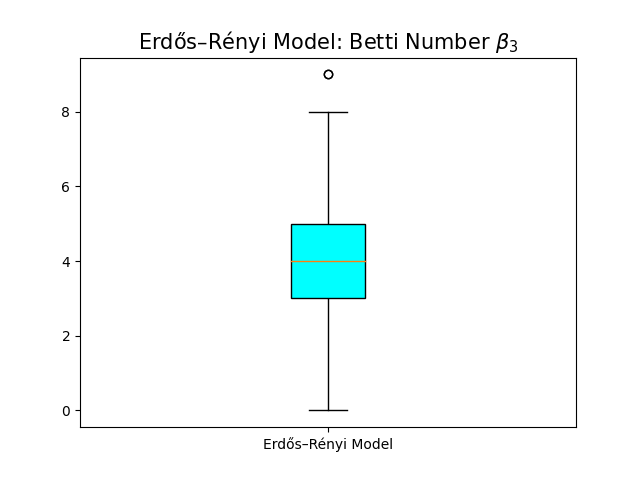
\includegraphics[width=7cm]{graph/betti3_er.png} }}%
    \qquad
    \subfloat[\centering Configuration Model]{{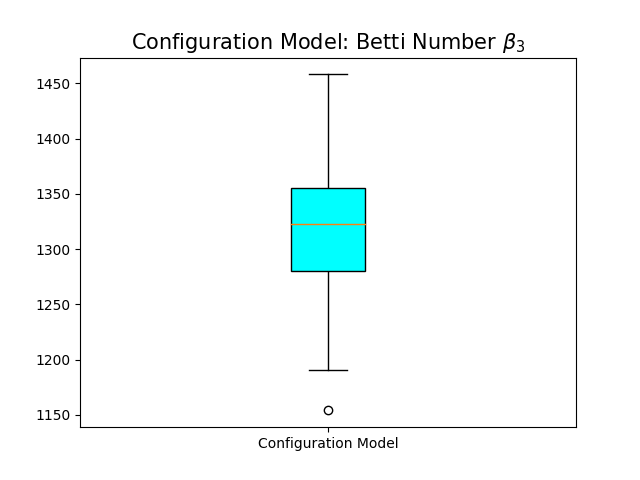
\includegraphics[width=7cm]{graph/betti3_conf.png} }}%
    \caption{Box-plots of Betti Numbers observed in the $3^{rd}$ dimension for the models}%
    \label{fig:example}%
\end{figure}

\begin{figure}[H]%
    \centering
    \captionsetup{justification=centering}
    \subfloat[\centering Geometric Configuration Model]{{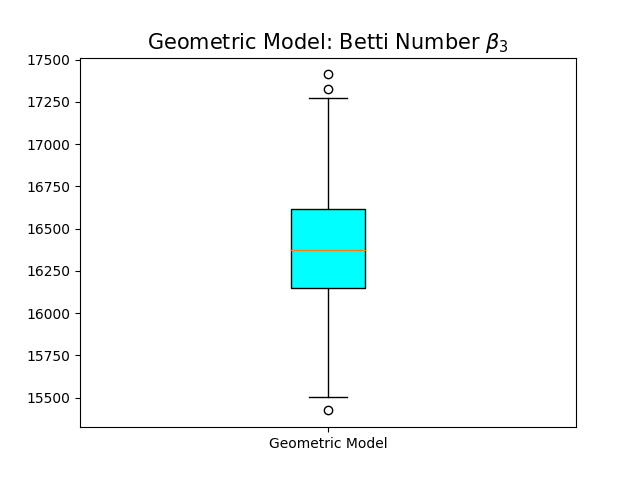
\includegraphics[width=7cm]{graph/betti3_geo.png} }}%
    \qquad
    \subfloat[\centering Block Configuration Model]{{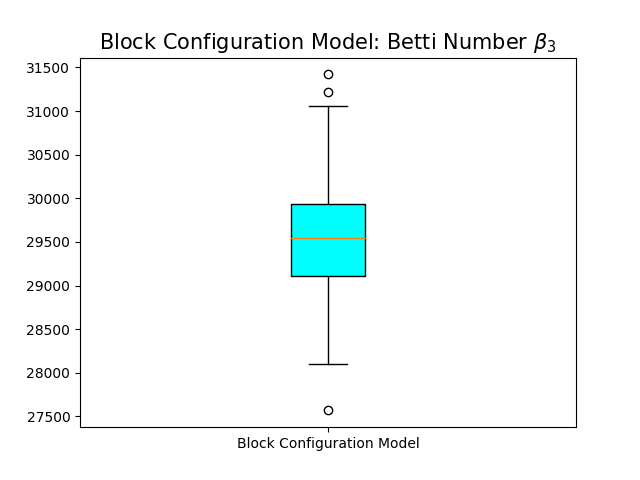
\includegraphics[width=7cm]{graph/betti3_block_conf.png} }}%
    \caption{Box-plots of Betti Numbers observed in the $3^{rd}$ dimension for the models}%
    \label{fig:example}%
\end{figure}

\begin{figure}[H]%
    \centering
    \captionsetup{justification=centering}
    \subfloat[\centering Block Geometric Configuration Model]{{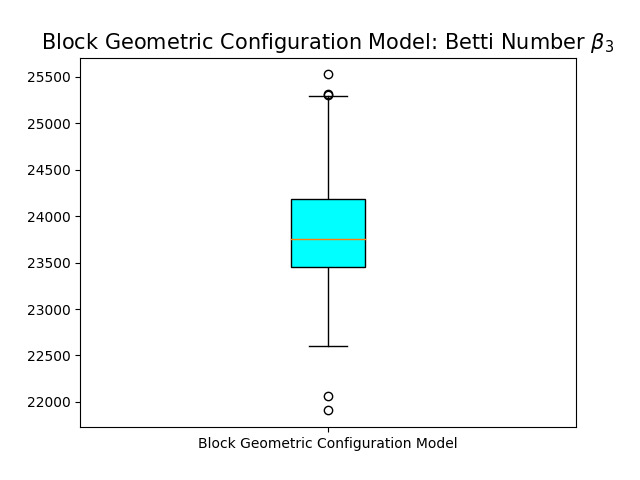
\includegraphics[width=7cm]{graph/betti3_block_geo.png} }}%
    \qquad
    \subfloat[\centering All Models]{{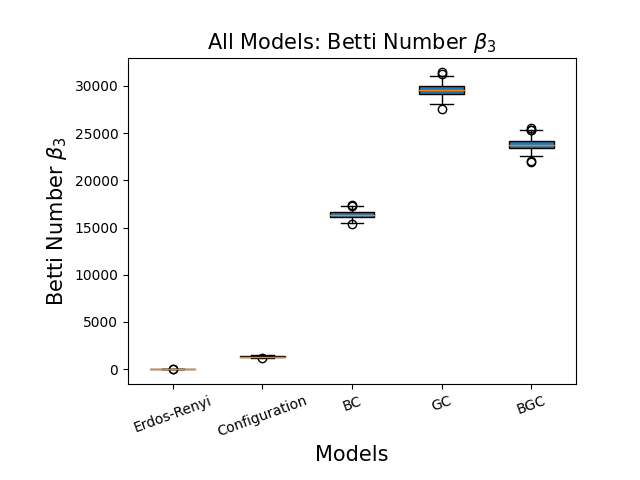
\includegraphics[width=7cm]{graph/all_betti.png} }}%
    \caption{Box-plots of Betti Numbers observed in the $3^{rd}$ dimension for the models}%
    \label{fig:example}%
\end{figure}


We also compare the $3^{rd}$ Betti Number with the Euler Characteristic for our 4 models. We can see that they cluster together within each model with a larger variation in the Betti Number. The block models observed similar values with respect to one another, especially in comparison to the other two models. The size of the graph can clearly give large differences in their clustered values as we see from the Configuration and Geometric Configuration models.

\begin{figure}[H]
\begin{center}
\captionsetup{justification=centering}
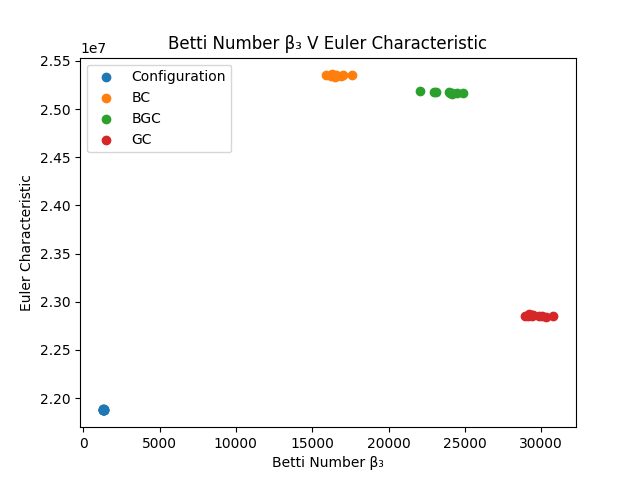
\includegraphics[width=12cm]{graph/bVe.png}
\caption{Betti number in dimension 3 against Euler characteristic}
\end{center}
\end{figure}

\subsection{Total Variation distance: Distance Distribution}
One of the statistics we mention in Section 2, Mathematical Preliminaries, is the Total Variation (TV) distance. We use this statistic to give us a measure of how well one model may fit to that of the Bio-M MC in various statistical measures. However, here, we use it to check the fit of distance distributions and in the next subsection, how well the Block-wise Edge densities fit for each model.

So, we ran 100 realisations of each model with the intent to see how well the distributions of each model fit the distribution of the Bio-M MC. Below, after 100 realisations of each model, we have a table of the mean of each distribution.

We can see that the models observed a wide range of TV distances in relation to one another, with the \ER model being the weakest and the GB model being the strongest. As mentioned in their respective sections, the BC model and the BGC model observe remarkably similar TV distances when comparing to the Bio-M MC. The spread of values for each respective model, was rather small, suggesting some consistency in the way the models reconnect the neurons in the MC.
\begin{center}
 \begin{tabular}{| c | c |}
 \hline
 \textbf{Model} & \textbf{Mean Total Variation distance}  \\ [0.5ex]
 \hline
 \ER &  0.7092   \\
 \hline
 Configuration & 0.6595    \\
 \hline
 Geometric Configuration & 0.3169   \\
 \hline
 Block Configuration & 0.3939   \\
 \hline
 Block Geometric Configuration & 0.3937 \\
 \hline
 General Biological & 1.5341e-08  \\
 \hline
\end{tabular}
\end{center}

\begin{figure}[H]%
    \centering
    \captionsetup{justification=centering}
    \subfloat[\centering \ER Model ]{{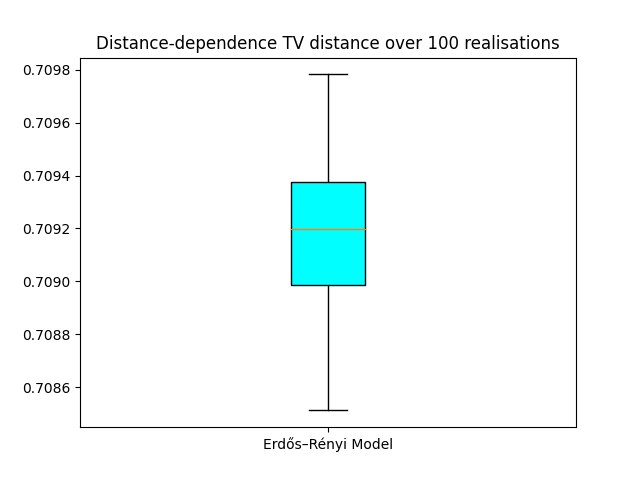
\includegraphics[width=7cm]{results_imgs/erModel.png} }}%
    \qquad
    \subfloat[\centering Configuration Model]{{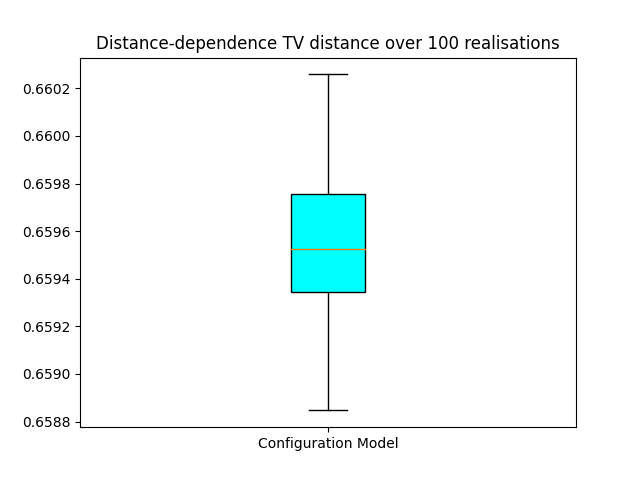
\includegraphics[width=7cm]{results_imgs/cModel.png} }}%
    \caption{Box-plots of observed total distance variation from each model to the Bio-M MC}%
    \label{fig:example}%
\end{figure}

\begin{figure}[H]%
    \centering
    \captionsetup{justification=centering}
    \subfloat[\centering Geometric Configuration Model]{{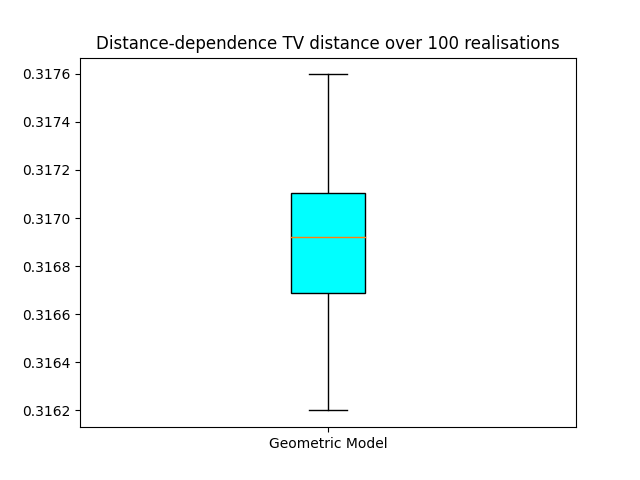
\includegraphics[width=7cm]{results_imgs/gcModel.png} }}%
    \qquad
    \subfloat[\centering Block Configuration Model]{{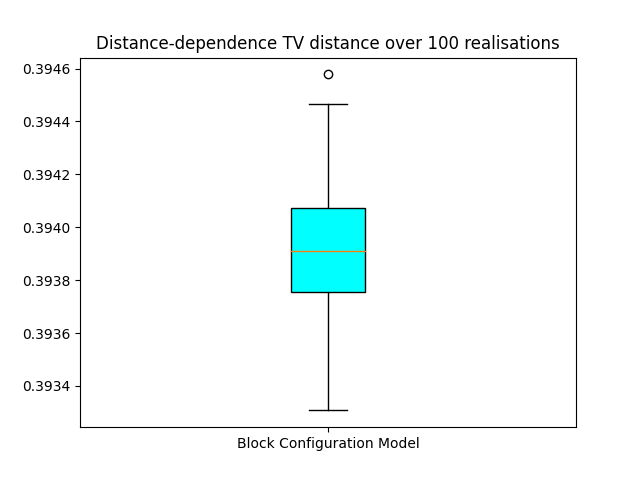
\includegraphics[width=7cm]{results_imgs/bcModel.png} }}%
    \caption{Box-plots of observed total distance variation from each model to the Bio-M MC}%
    \label{fig:example}%
\end{figure}

\begin{figure}[H]%
    \centering
    \captionsetup{justification=centering}
    \subfloat[\centering Block Geometric Configuration Model]{{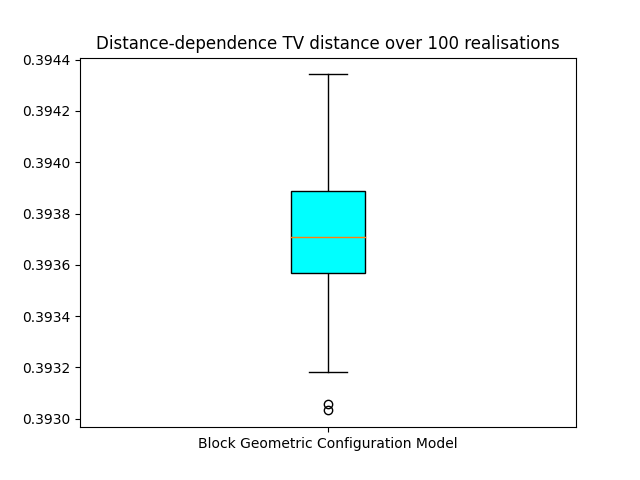
\includegraphics[width=7cm]{results_imgs/bgcModel.png} }}%
    \qquad
    \subfloat[\centering General Biological Model]{{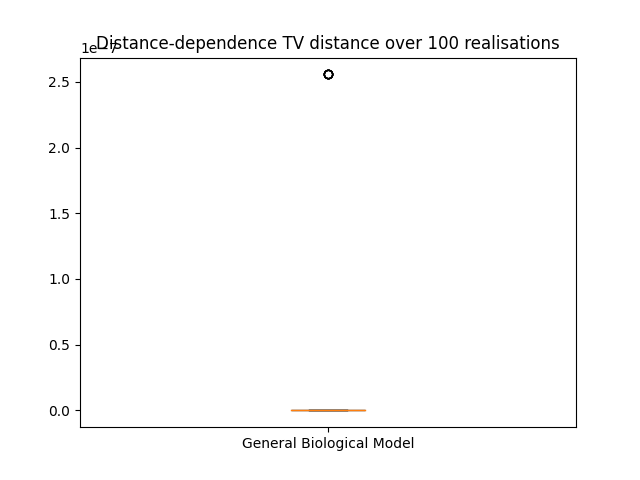
\includegraphics[width=7cm]{results_imgs/gbModel.png} }}%
    \caption{Box-plots of observed total distance variation from each model to the Bio-M MC}%
    \label{fig:example}%
\end{figure}
A note on the General Biological model from what we see in Figure 46(b) is that over the 100 realisations we obtained a TV distance greater than zero for one realisation. Given that this occurred only once and that the difference is insignificant, we do not concern ourselves with this.

\subsection{Total Variation distance: Block-wise Edge Densities}
Here, we compare the Block-wise Edge densities between each model and the Bio-M MC. As we mentioned previously, there were 100 realisations of each model and each were compared to the Bio-M MC. To begin comparison, we compare each block and then sum over all blocks to ascertain the TV distance of each model to the Bio-M MC and where relevant, we then give a breakdown of TV distances, block by block.

\begin{figure}[H]%
    \centering
    \captionsetup{justification=centering}
    \subfloat[\centering \ER Model]{{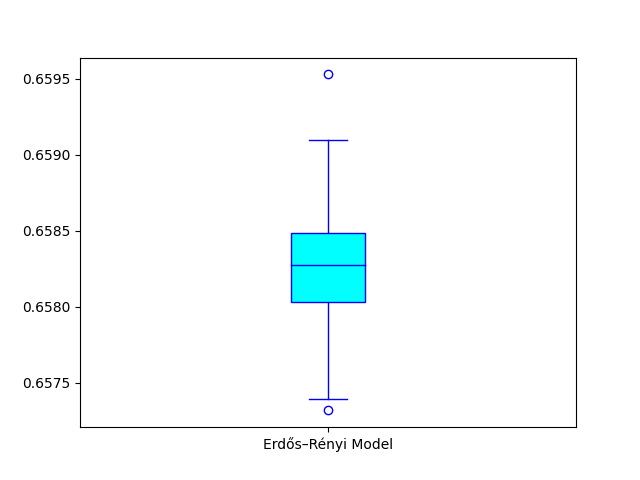
\includegraphics[width=7cm]{results_imgs/er_block_var.png} }}%
    \qquad
    \subfloat[\centering Configuration Model]{{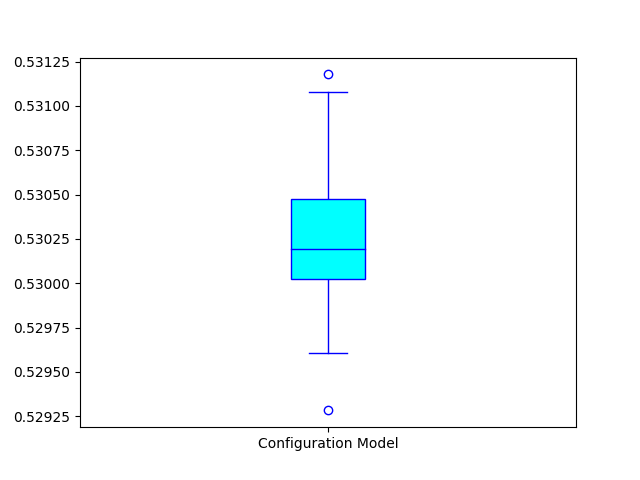
\includegraphics[width=7cm]{results_imgs/conf1_overall.png} }}%
    \caption{Box-plots of observed total distance variation from each model to the Bio-M MC}%
    \label{fig:example}%
\end{figure}
Figure 47 shows us the \ER model and the Configuration model. Both models show a similar range of values, however, the range of values given by the Configuration model is closer to that of the Bio-M MC. This 0.12 improvement between models is somewhat significant, highlighting the importance to maintain the in-degrees and out-degrees of the respective neurons in an already observed MC.

\begin{figure}[H]%
    \centering
    \captionsetup{justification=centering}
    \subfloat[\centering Geometric Configuration Model]{{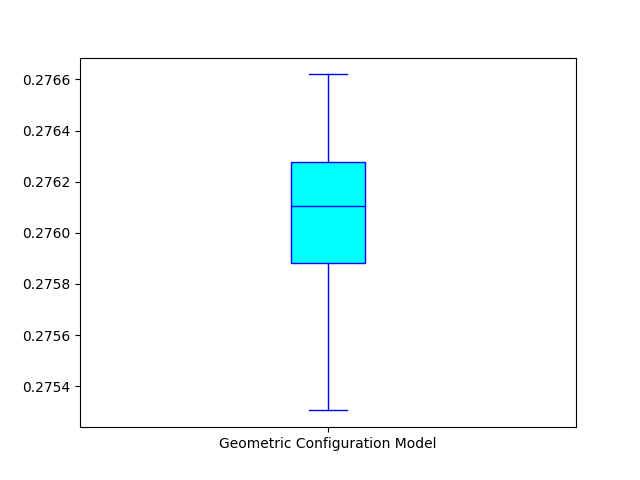
\includegraphics[width=7cm]{results_imgs/gc1_overall.png} }}%
    \qquad
    \subfloat[\centering Block Configuration Model]{{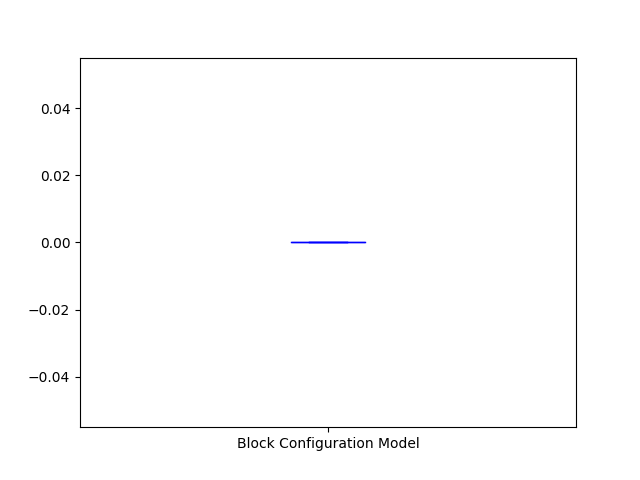
\includegraphics[width=7cm]{results_imgs/bc_block_var.png} }}%
    \caption{Box-plots of observed total distance variation from each model to the Bio-M MC}%
    \label{fig:example}%
\end{figure}

Figure 48(a) highlights further the importance of a geometric constraint applied to the MC. The improvement of Block-wise Edge densities almost doubles from the Configuration model. Furthermore, we have no outliers in our range of values, showing that the model can statistically be more consistent with the Bio-M MC. The Block Configuration model exhibits no differences to the Bio-M MC as is the case for the BGC model and the GB model. This is since they rearrange connections within the layer by layer blocks or subsets of these (morphological blocks).
\begin{figure}[H]%
    \centering
    \captionsetup{justification=centering}
    \subfloat[\centering Block Geometric Configuration Model]{{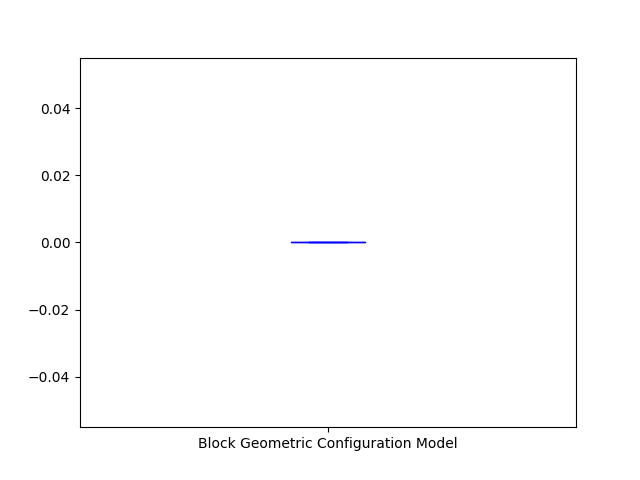
\includegraphics[width=7cm]{results_imgs/bgc_block_var.png} }}%
    \qquad
    \subfloat[\centering General Biological Model]{{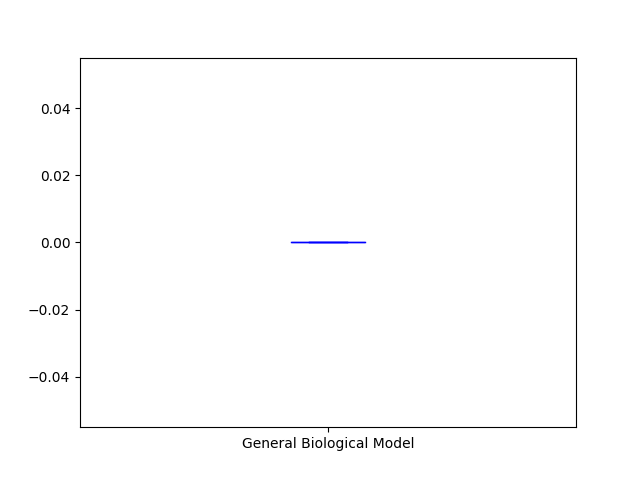
\includegraphics[width=7cm]{results_imgs/GB_block_var.png} }}%
    \caption{Box-plots of observed total distance variation from each model to the Bio-M MC}%
    \label{fig:example}%
\end{figure}


\begin{figure}[H]
\begin{center}
\captionsetup{justification=centering}
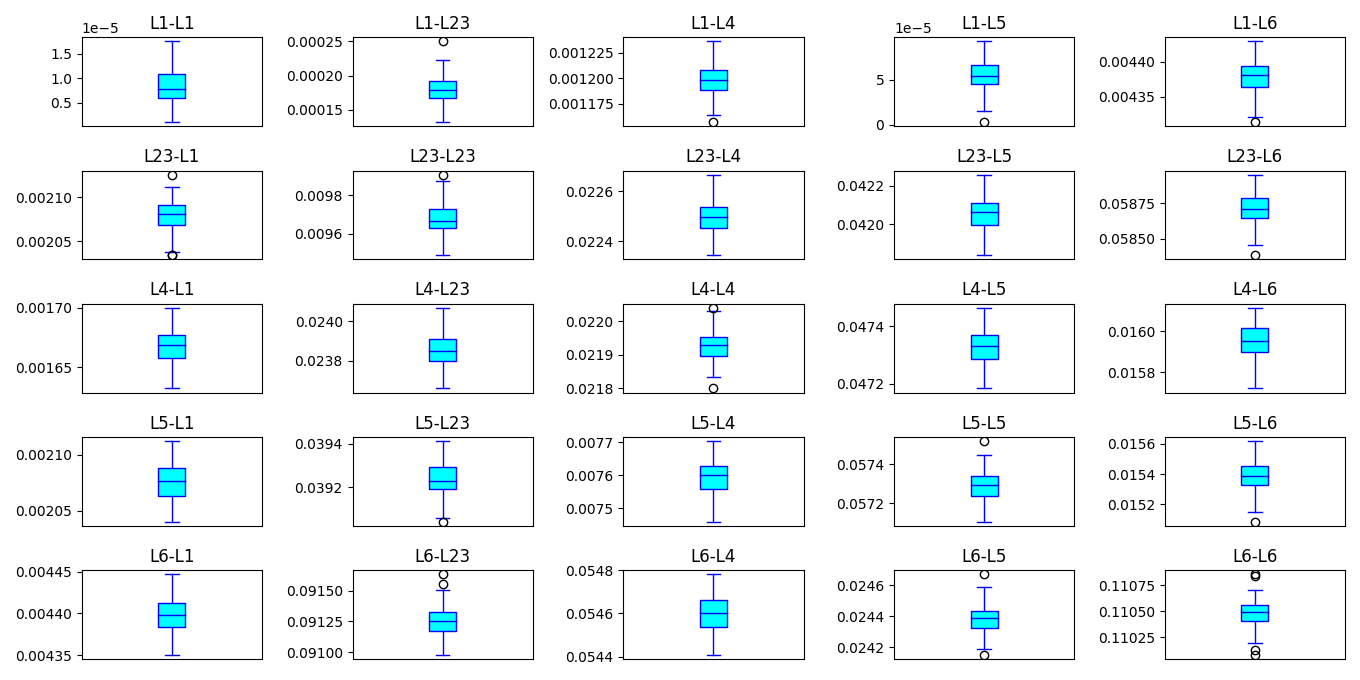
\includegraphics[width=12cm]{results_imgs/er_bed.png}
\caption{Block-wise Edge Density Total Variation Distance Block by Block: \ER Model}
\end{center}
\end{figure}
The \ER model gives a range of TV distances for each block. The biggest occurring in L6 to L6. The smallest sets of values occur in the blocks that relate to Layer 1, whether it be the pre-synaptic set of neurons or the post-synaptic set of neurons.
\begin{figure}[H]
\begin{center}
\captionsetup{justification=centering}
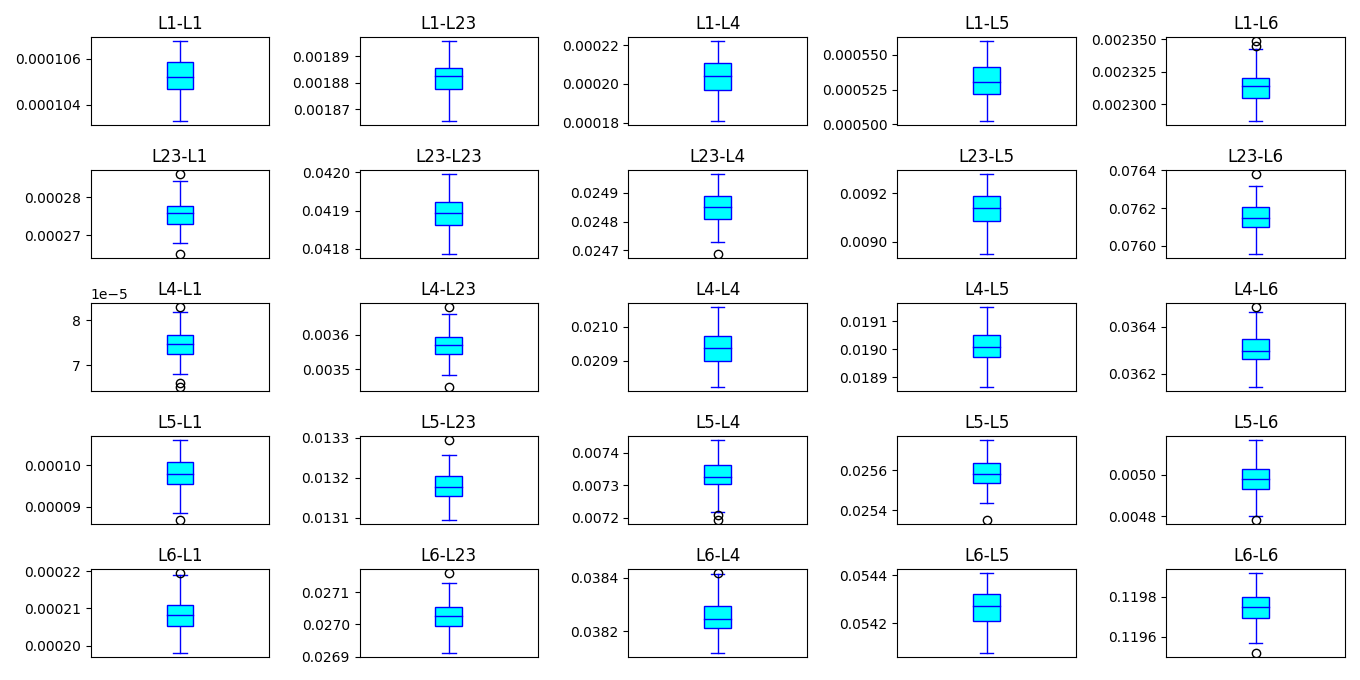
\includegraphics[width=12cm]{results_imgs/conf_bed.png}
\caption{Block-wise Edge Density Total Variation Distance Block by Block: Configuration Model}
\end{center}
\end{figure}
Now, likewise with the \ER model, the Configuration Model observes the largest set of TV distances from L6-L6 and similarly much smaller values for L1, whether it be from pre-synaptic neurons or to post-synaptic neurons, the TV distance values here are just a lot smaller.

\begin{figure}[H]
\begin{center}
\captionsetup{justification=centering}
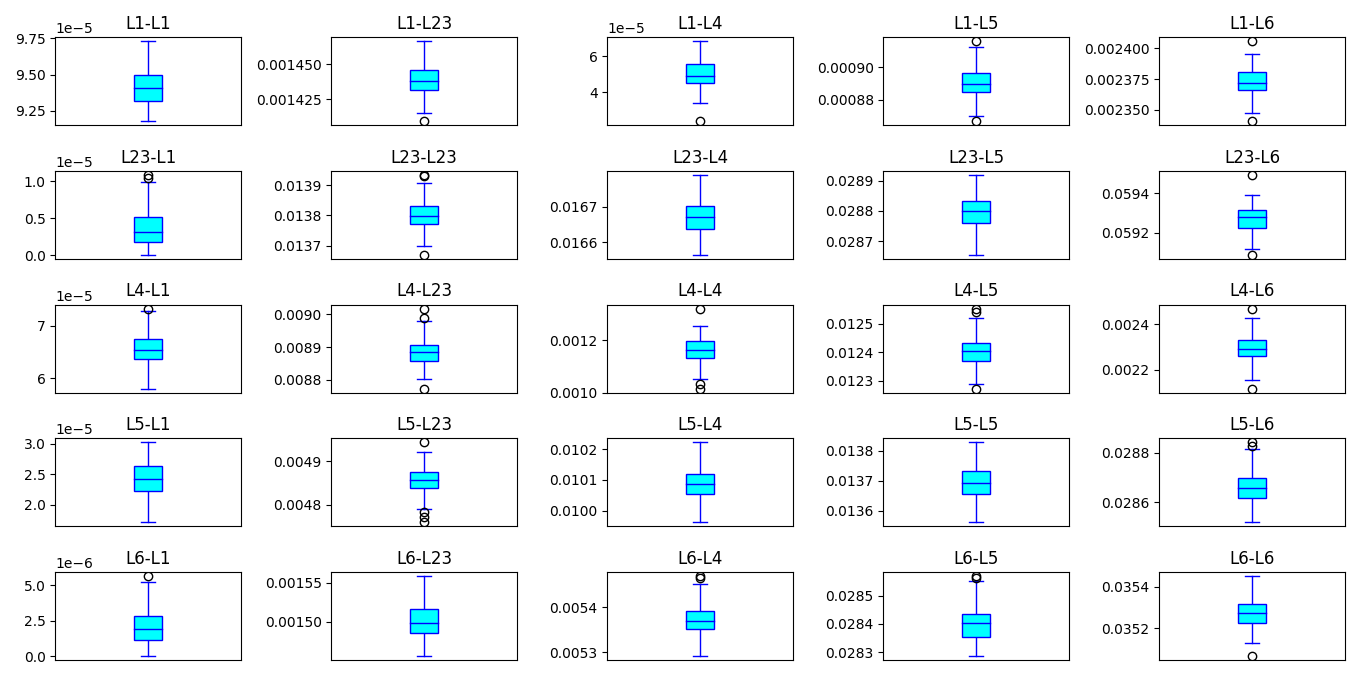
\includegraphics[width=12cm]{results_imgs/gc_bed.png}
\caption{Block-wise Edge Density Total Variation Distance Block by Block: Geometric Configuration Model}
\end{center}
\end{figure}
As mentioned for the \ER model and the Configuration model, the smallest differences occur in relation to neurons in Layer 1 for the GC model. However, we note here that in fact, there is a large improvement to the difference in respect of the L6-L6 connections, where we only see a mean TV distance of approximately 0.025, a large improvement on the previous two models, highlighting the strength of the geometric constraint.


\subsection{Timings}
\begin{figure}[H]
\begin{center}
\captionsetup{justification=centering}
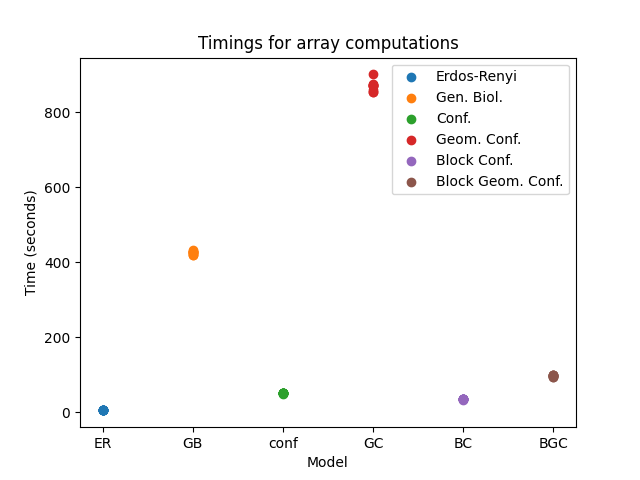
\includegraphics[width=12cm]{graph/timings.png}
\caption{Computation times for the random graphs}
\end{center}
\end{figure}

\begin{center}
 \begin{tabular}{| c | c | c | c |}
 \hline
 \textbf{Model} & \textbf{Min(s)} & \textbf{Mean(s)} & \textbf{Max(s)} \\ [0.5ex]
 \hline
 \ER & 5 & 5    & 5    \\
 \hline
 Configuration &  49.78 & 50.63  & 51.75   \\
 \hline
 Geometric Configuration & 854.87
 & 870.93 &  901.63   \\
 \hline
 Block Configuration & 34.77 & 34.01 & 35.55   \\
 \hline
 Block Geometric Configuration & 94.77
  & 97.55 & 99.89 \\
 \hline
 General Biological & 420  & 426     & 432   \\
 \hline
\end{tabular}
\end{center}
Finally, we have our timings for the models. All of these were computed on the same machine, of which the details are listed below. However, there were slight differences in the methods between my models and that of the General Biological model and Bio-M MC. The General Biological model and Bio-M MC were computed first by converting the file formats from H5 to CSV and then converted to an NPY array, whereas my models just simply needed to take the saved NPY array.

A note on the geometrically constrained models is that they had a similar computation time up until approximately 80$\%$ completion and then slowed down significantly in order to connect the remaining vertices. Therefore the remaining 20$\%$ of connections took the majority of time to compute.
\newpage
\begin{lstlisting}[language=bash]
Architecture:                    x86_64
CPU op-mode(s):                  32-bit, 64-bit
Byte Order:                      Little Endian
Address sizes:                   43 bits physical, 48 bits virtual
CPU(s):                          12
On-line CPU(s) list:             0-11
Thread(s) per core:              2
Core(s) per socket:              6
Socket(s):                       1
NUMA node(s):                    1
Vendor ID:                       AuthenticAMD
CPU family:                      23
Model:                           113
Model name:                      AMD Ryzen 5 3600 6-Core Processor
Stepping:                        0
Frequency boost:                 enabled
CPU MHz:                         2199.811
CPU max MHz:                     3600,0000
CPU min MHz:                     2200,0000
BogoMIPS:                        7199.87
Virtualization:                  AMD-V
L1d cache:                       192 KiB
L1i cache:                       192 KiB
L2 cache:                        3 MiB
L3 cache:                        32 MiB
NUMA node0 CPU(s):               0-11
\end{lstlisting}





